\section{Final System Architecture and Design}

The final system architecture is a three layered architecture. Its top UI layer is built using React JS with its middle layer built upon Node JS and its bottom layer a NOSQL database using Firebase. Each layer can communicate with the layer next to it, with the user only interacting with the top layer. We chose react as it is the industry standard for front end javascript development and pairs very well with Node JS. Node JS was similarly chosen for its strong pairing with react and its performance for real time data communication, making it perfect for a multiplayer game. Firebase was chosen for its ease of use as well as its performance and scalability in comparison to its SQL counterparts. For our class architecture, we have a user class, made up of all of the users information such as name, email and balance. Users have messages and stats, and when entering a game a player is made from the users information. Players can then interact with the game and have cards and can draw more from the deck. Additionally the admin class extends the user class and provides an additional level of access to the system.\ref{fig:uml_diagram}


\begin{figure}[H]
    \centering
    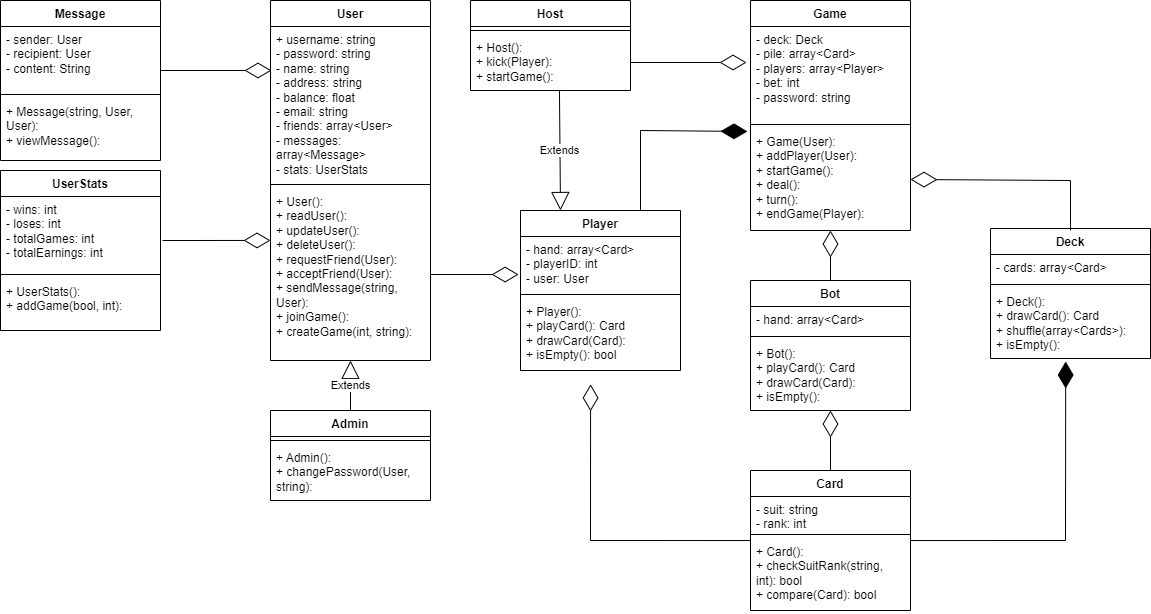
\includegraphics[width=\textwidth]{Crazy8sUML.png}
    \caption{UML Diagram of the Final System Architecture}
    \label{fig:uml_diagram}
\end{figure}